\documentclass[a4paper,12pt]{ltjsarticle}
\usepackage{luatexja}
\usepackage[no-math]{luatexja-fontspec}
\usepackage{luatexja-preset}
\usepackage{amsmath}
\usepackage{amsfonts}
\usepackage{amssymb}
\usepackage{graphicx}
\usepackage{multicol}
\usepackage{xcolor}
\usepackage{tabularx}
\usepackage{url}
\usepackage{pdfpages}
\usepackage[normalem]{ulem}
\usepackage[top=13mm,bottom=20mm,left=20mm,right=20mm]{geometry}

\setmainfont{Arimo}
\setsansfont{Arimo}

\begin{document}

% ---------------Header---------------
\pagestyle{empty}
\begin{multicols}{2}
\setlength{\columnsep}{4pt}
\setlength{\tabcolsep}{2pt}

% ---------------TItle---------------
\huge
\noindent
\textsf{Shunsuke Fujisawa}\par\noindent
\textsf{藤澤 俊祐}\par\noindent
\columnbreak
\normalsize
\color{gray}
Technical Consaltant at UiPath K.K.\par\noindent
\color{black}
\small
\begin{tabularx}{0.9\linewidth}{lX}
Address:&1-5-11 Nishitomi Fujisawa-shi Kanagawa, Japan, 2510001\\
Phone:& (+81)90-5523-6484\\
Email:&seekworser1963@gmail.com\\
\color{white}
\colorbox{black}{\textsf{in}}&\url{https://www.linkedin.com/in/fujisawa-shunsuke/}
\end{tabularx}
\end{multicols}

% ---------------Summary---------------
\Large\noindent
\uline{\textsf{Summary}\hspace{\fill}}
\normalsize\par\noindent

\begin{itemize}
    \item 2-years experience as technical consaltant
    \item Education on physics, mathematics and computer science.
\end{itemize}

% ---------------Key Skills---------------
\Large\noindent
\uline{\textsf{Key Skills}\hspace{\fill}}
\normalsize\par\noindent
\begin{tabularx}{0.9\linewidth}{lX}
    Language:&Japanese (mother tongue), English (fluent in business situations, TOEIC Score: 820)\\
    Programming:&VB.NET, C\#, Python, MATLAB, Fortran, C++, Java, LaTeX, VHDL, VISA (experienced), JavaScript/TypeScript, LabView (knowledgeable)
\end{tabularx}

% ---------------Work Experience---------------
\Large\noindent
\uline{\textsf{Work Experience}\hspace{\fill}}
\normalsize\par\noindent\vspace{-12pt}\par\noindent
\large\noindent
\textsf{2020-present\hspace{1cm}UiPath K.K.\hspace{1cm}Chiyoda-Ku, Tokyo}
\normalsize\par
Technical Consultant, RPA Developer
\begin{itemize}
    \item Designed and developed RPA which is utilized in customer environment
    \item Provided customer support about the owning products
    \item Build and maintain verification envirionment (VMs on VMware).
    \item Assigned to the one of the biggest banking company client and mainly handle customer facing tasks for my own.
    \item Communicating with development teams about feedbacks about the products
\end{itemize}

% ---------------Education---------------
\Large\noindent
\uline{\textsf{Education}\hspace{\fill}}
\normalsize\par\noindent\vspace{-12pt}\par\noindent
\large\noindent
\textsf{Master of Science (physics), The University of Tokyo in Mar. 2019.}
\normalsize
\begin{itemize}
    \item Engaged in improving measurement performance using mathematical optimization and proposed the framework to expand the bandwidth of measurement.
    \item Used Python for processing measurement data and making graphs for journal.
    \item Supported the research of other students by developing software, advising on programming and setting up the computers.
\end{itemize}
\large\noindent
\textsf{Bachelor of Liberal Arts, The University of Tokyo in Mar. 2017.}
\normalsize
\begin{itemize}
    \item Modified an existing algorithm for specific situation and evaluated its performance.
    \item Inplemented the algrithms using Fortran.
\end{itemize}

\newpage

% \topskip0pt
% \vspace*{\fill}
\vspace*{40pt}
\huge
\begin{center}
    Appendix
\end{center}
\normalsize
\begin{enumerate}
    \item Paper which I wrote in my master course
    \item Poster in QIT40
\end{enumerate}
% \vspace*{\fill}

\newpage

\addtolength{\oddsidemargin}{0pt}
\addtolength{\evensidemargin}{0pt}
\addtolength{\topmargin}{0pt}
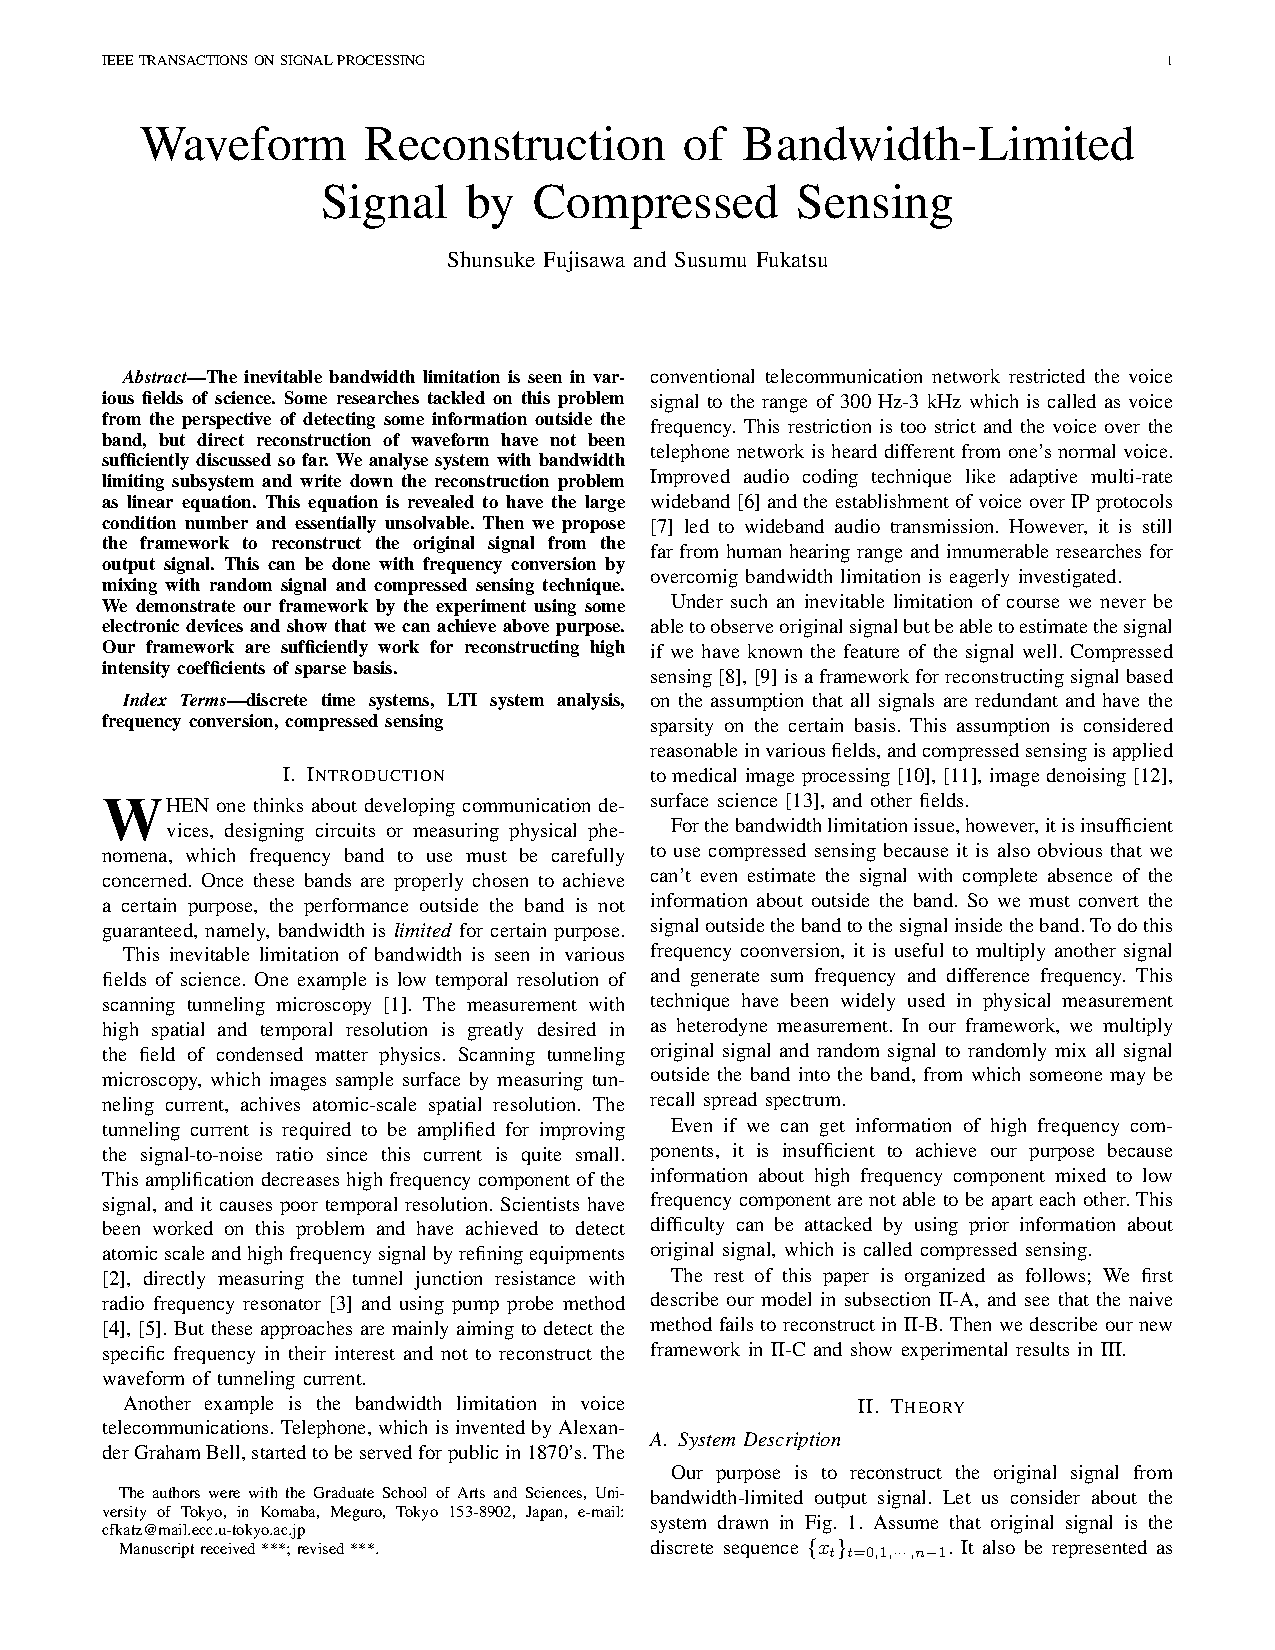
\includepdf[pages={1-}, scale=0.98]{figure/heterodyne_cs_paper.pdf}

\end{document}